How to line up columns...you have to manually line up the columns if they are not automatically aligned after copy. Usually the heading has to be adjusted.

\begin{lstlisting}[escapeinside={¿}{¿},frame=single,breaklines,columns=fixed]
¿\tld¿ ps
PID   TTY      TIME     CMD
11875 pts/1    00:00:00 ps
31589 pts/1    00:00:00 bash 
\end{lstlisting}



\includegraphics[width=.6cm]{figures/internalhyperlink}

\includegraphics[width=.6cm]{figures/globe}

Uncommented shebang in code
¿\#¿!/bin/bash

Indent block of text
\begin{addmargin}[1em]{2em}
\end{addmargin}

How to type an inverted question mark in the main body....
{?`}
{?`}{\{-}\}{?`} produces ¿{-}¿

Exempt literal # in lstlisting
¿\tbi{\#}¿

¿\textcolor{red}{How to manage repositories} \textcolor¿
¿\textit{\color{red}How to manage repositories}¿

To do
\todo[inline]{create ans ch 2}

Insert color heading in tabularx
\textit{\color{red}Search for a string and delete the files containing that string} & four different methods are shown.\\

Symbolic link colors in code
[~] ls -la /usr/sbin/telinit
lrwxrwxrwx. 1 root root 16 Feb  1 06:04 ¿\textbf{\color{Aquamarine}/usr/sbin/telinit}¿ -> ¿\textbf{\color{green}../bin/systemctl}¿

Insert a picture
\includegraphics[width=0.2\textwidth]{figures/logo_lftcert_sysadmin}\\[1cm] 

Pictures for external and internal hyperlinks

\includegraphics[width=.6cm]{figures/globe} The description below is taken from \href{https://fedoraproject.org/wiki/SELinux_FAQ}{SELinux FAQ}.\\


\includegraphics[width=.6cm]{figures/internalhyperlink}

Figures and listing figures as an index. At end of main.tex, you have to call the \listoffigures to create the figures appendix.

\begin{figure}[!h]
\centering
\href{https://en.wikipedia.org/wiki/Luddite}{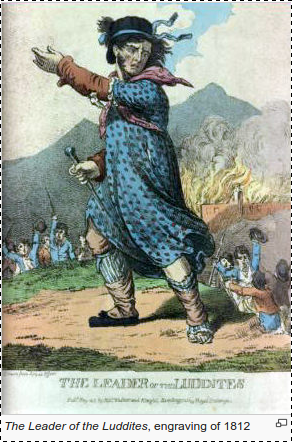
\includegraphics[width=0.2\textwidth]{figures/ludite_leader}}
\caption{The leader of the Ludites}
\label{title_page_1_ludites}
\end{figure}

Without the use of {figure}, just insert the image.

\href{https://en.wikipedia.org/wiki/Luddite}{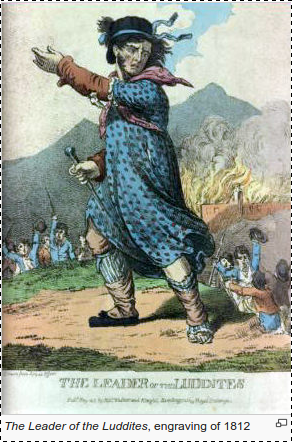
\includegraphics[width=0.2\textwidth]{figures/ludite_leader}}\\[1cm]

Challenge...\todo[inline]{mang modify function to remove last line - second header}

Internal hyperlinks1 - within code
¿\textbf{\color{red}Challenge:} How would you do that? \hyperlink{sedel}{Answer.}¿

\hypertarget{sedel}{Processes - Breaking a complex command into parts}

\begin{minted}[frame=single,breaklines]{bash}
[~] w | awk '{print $2}' | sed '1,2d'
\end{minted}

Internal hyperlinks 2 - regular LaTeX

Destination (where you go when you click the hyperlink): \subsection{Aliases}\label{subsec:aliases}

Source link (The hyperlink that you click to get to the destination.): \hyperref[subsec:aliases]{aliases}
Of course, you would use 'sec' instead of 'subsec' for section headers.

Note: within code, you have to surround these items with the escape inside character.

¿\hyperref[subsec:aliases]{aliases}¿

Internal hyperlinks within code...bounded by comments.
#
Or, go there |\hyperref[subsec:finduserprocs]{now}|.
#

\begin{minted}[frame=single,breaklines]{bash}
\end{minted}

\begin{tabularx}{\linewidth}{>{\bfseries}X | X} % the X is needed to wrap text
\caption{Manpages}\label{table:groups-examples}\\ % title of Table
\toprule
\normalfont{Command} & Action \\% inserts table heading, unbolds 1st column heading
\midrule
groupadd -g 1111 mygrp & create a new group called \tqs{mygrp} with GID of 1111. Note, user created groups will always start above GID 1000. You do not have to specify the GID as it is automatically created.\\[2mm]
ps -ef | grep -E 'tty|pts' & create a new group called \tqs{my2grp} that has the same GID as \tqs{mygrp}\\[2mm]	
\bottomrule
\end{tabularx}


\begin{itemize}
	\item \tbi{} 
\end{itemize}

No bullets
\begin{itemize}
	\item[] \tbi{} 
\end{itemize}

\begin{enumerate}
	\item{high-ordered-bit sum for special permissions: SUID, GID, sticky bit}
	\item{user owner - read bit}
\end{enumerate}

https://en.wikipedia.org/wiki/List_of_Unicode_characters

Include Latex inside minted using a single pipe symbol as the escape symbol. I tried the upside down question mark, but that did not work. ctrl+shift+u 00bf

\begin{minted}[escapeinside=||,mathescape=true,frame=single,breaklines]{python}
|\tbi{\textcolor{red}{user:mgd:rw-}}|
\end{minted}

\begin{minted}[escapeinside=\{\},frame=single,breaklines]{bash}
With this latter statement, you only need to enclose your LaTeX code between {} not \{\}.
\end{minted}

Include LateX inside lstlisting ... no code specified

\begin{lstlisting}[escapeinside={*@}{*@},frame=single,breaklines]
	then precede code with *@ and terminate with *@
	
\begin{lstlisting}[escapeinside={¿}{¿},frame=single,breaklines,columns=fixed]
	then precede code with ¿ and terminate with ¿
	ctrl+shift+u 00bf at command line
Here is an example of a comment in red!	
# ¿\color{red}{Tr\'es cool! Command redirection rocks!}¿ 
# ¿\textbf{\color{red}Challenge:} How would you order the list alphabetically sorted by file extension? \hyperlink{sortbyfileext}{Answer}¿ 	
\end{lstlisting}

And if I want to include a whole source code file, I use the lstinputlisting command:

\lstinputlisting{../Matlab/inverse/MetropolisDataMany.m}

Note: if trying to line up a grep of a manpage, use the spacebar to align text, don't use tabs
\begin{verbatim}
\end{verbatim}

CTRL+SHIFT+u and then release and then type in a ascii hex number

{accents} is about diacritics, i.e., ancillary glyphs added to a letter, or basic glyph. Some diacritical marks, such as the acute ( ´ ) and grave ( ` ), are often called accents. Diacritical marks may appear above, below, or within a letter, or between two letters.

accents is about diacritics, i.e., ancillary glyphs added to a letter, or basic glyph. Some diacritical marks, such as the acute ( ´ ) and grave ( ` ), are often called accents. Diacritical marks may appear above, below, or within a letter, or between two letters.

Text mode

Plain TeX makes it possible to typeset the most commonly used accents:

\` (grave accent): à

\' (acute accent): á  minted escapeinde=|| |Tr\'es| generates  Trés

\^ (circumflex or “hat”): â

\" (umlaut or dieresis): ä

\~ (tilde or “squiggle”): ã

\= (macron or “bar”): ā

\. (dot accent): ȧ

\u (breve accent): ă

\v (háček or “check”): ǎ

\H (long Hungarian umlaut): ő

\t (tie-after accent): a͡

\c (cedilla): ş

\d (dot-under accent): ạ

\b (bar-under accent): ο̩

\k (ogonek): ą

The Unicode character encoding UTF8 includes several special characters and characters with accents. The following code specifies that the encoding of the LaTeX document source file is UTF8. As font encoding is specified T1, because it supports the encoding of extended character sets in fonts:

\usepackage[utf8]{inputenc}
\usepackage[T1]{fontenc}

Of course, the encoding in the text editor needs to be set to utf8, as well.

Math mode

The following commands may be used only in math mode to produce accents;

\hat{o} (circumflex): enter image description here
\widehat{oo} (wide version of \hat over several letters): enter image description here
\check{o} (vee or check): enter image description here
\tilde{o} (tilde) enter image description here
\widetilde{oo} (wide tilde) enter image description here
\acute{o} (acute accent): enter image description here
\grave{o} (grave accent): enter image description here
\dot{o} (dot over the letter): enter image description here
\ddot{o} (two dots over the letter): enter image description here
\breve{o} (breve): enter image description here
\bar{o} (macron): enter image description here
\vec{o} (vector (arrow) over the letter): enter image description here

Opening videos, pdf, png

Note, the following links do not work in TexWorks, but they do work within 'main.pdf'.\\
Open a video on Fedora with VLC, \href{run:attachments/video.mp4}{myvideo}.\\
Open a picture on Fedora with Shotwell, \href{run:attachments/texworks.png}{mypng}.\\
Open a PDF on Fedora with Evince, \href{file://attachments/sharp.pdf}{mypdf}.

%% hyperef package

1. Define a label...
\section{Math symbols} \label{math_msymb}

2. Reference the label...
\autoref{math_msymb} 

3. What appears in text is a hyperlink called: section 2.4, not Math symbols...

The package \imp{hyperref} is the package for referring to labeled elements of a document and hyperlinks. Now, chapters, sections, equations, figures, tables and other elements can be labeled and referred to, e.g., \autoref{math_fe}, \autoref{math_msymb} and \autoref{href}. These are clickable links which in the pdf redirects the reader to the referred element (with ALT+LEFT you can then go back to where you were reading). Here, different alternatives can be used, e.g., \ref{href}, \autoref{href} or \hyperref[href]{Chapter \ref*{href}}. Depending on which language you have to write something, you may need language options (e.g., ngerman for German hyperlinks).

1. Macros
%% Name references
% http://tex.stackexchange.com/questions/178720/reference-chapter-number
% The following was how the command appeared on the webpage, I modified it. Note, in the commented command, the space before the \nameref is a hardspace between the two items.
%\NewDocumentCommand{\chapref}{s m}{\autoref{#2}\IfBooleanF{#1} { \nameref{#2}}}
\newcommand{\chapref}[1]{\autoref{#1}. \nameref{#1}}
% http://stackoverflow.com/questions/1491842/references-with-text-in-latex
\newcommand{\secref}[1]{\autoref{#1}. \nameref{#1}}

2. Labels in document
% A chapter label.
\chapter{Where for to, me trout?}
\label{ch:intro}
% A section label.
\section{What's it all about Murray?}
\label{sec:allabout}

3. Reference in another part of document
Internal Hyper reference: \hyperref[sec:allabout]{About}\\
Internal Auto reference with section number: \autoref{sec:allabout}\\
Internal Auto reference with with Chapter Number, Chapter Title; Section Number, Section Title: \chapref{ch:intro} \secref{sec:allabout}

4. How it appears in PDF...as hyperlinks after the :
Internal Hyper reference: About
Internal Auto reference with section number: section 1.10
Internal Auto reference with with Chapter Number, Chapter Title; Section Number, Section Title:
chapter 1. Where for to, me trout? section 1.10. What’s it all about Murray?

Table with long commands
\begin{table}[!h]  % maybe \begin{table}[!htpb]
\caption{Using \emph{top} at the command line}
\begin{tabular}{|>{\bfseries}l p{12cm}|} % \begin{tabular}{|>{\bfseries}l p{8cm}|}
\hline
\normalfont{Command} & Action \\\hline
top -n1 -b | head -10 & Run only one iteration of the \emph{top} command. This prints 10 lines which results in only the top 3 processes listed due to 5 lines for heading, a blank line, and then the table heading. So, only 3 lines left for the process list. If you use this method, add \# of processes you want to 7 for the \emph{head} option. This issue is addressed in the next command.\\[3mm]
top -b -d5 -n10 -u mgc & Run 10 iterations of \emph{top} with a 5 second delay for user \emph{mgc}. All processes are listed for \emph{mgc}, 10 distinct \emph{top} tables are generated. Each table has the 5 lines of information that the \emph{top} ncurses window provides.\\[3mm]
\multicolumn{2}{|l|}{\textbf{top -n1 | egrep -v "top|Tasks|Cpu|Mem|Swap"}}\\
& Run 1 iteration of the \emph{top} command, but remove the top 5 lines of information, that is, the lines beginning with these keywords.\\[3mm]	
\multicolumn{2}{|l|}{\textbf{top | egrep -v "top|Tasks|Cpu|Mem|Swap|PID" | tee -a top.log}}\\
& Run and display the \emph{top} command until you manually end the command...and \emph{tee} the output to the file \textsl{top.log}, remove the top five lines of information and the table headings.\\[3mm]
\hline
\end{tabular}
\end{table}